%! Author = drakanoy
%! Date = 10.09.2024

% Preamble
\documentclass[12pt]{article}

% Packages
\usepackage[utf8]{inputenc}
\usepackage[T2A]{fontenc}
\usepackage[english, russian]{babel}
\usepackage[a4paper, includefoot, left=1.5cm, right=1.5cm, top=1cm, bottom=1.5cm, headsep=1cm, footskip=1cm]{geometry}
\usepackage{makecell}
\usepackage{amsmath}
\usepackage{graphicx}
\usepackage{enumitem}
\usepackage{svg}
\usepackage{multirow}
\usepackage{hyperref}
\usepackage{mathtools}
\usepackage{amssymb}
\usepackage{textcomp}

% Document
\begin{document}
\begin{large}
\begin{center}
\LARGE \textbf{Домашняя работа}
\par
\LARGE \textbf{Кононов Александр Михайлович}
\par
    \textbf{25.09.2024}
\end{center}
\par Условие:
\par
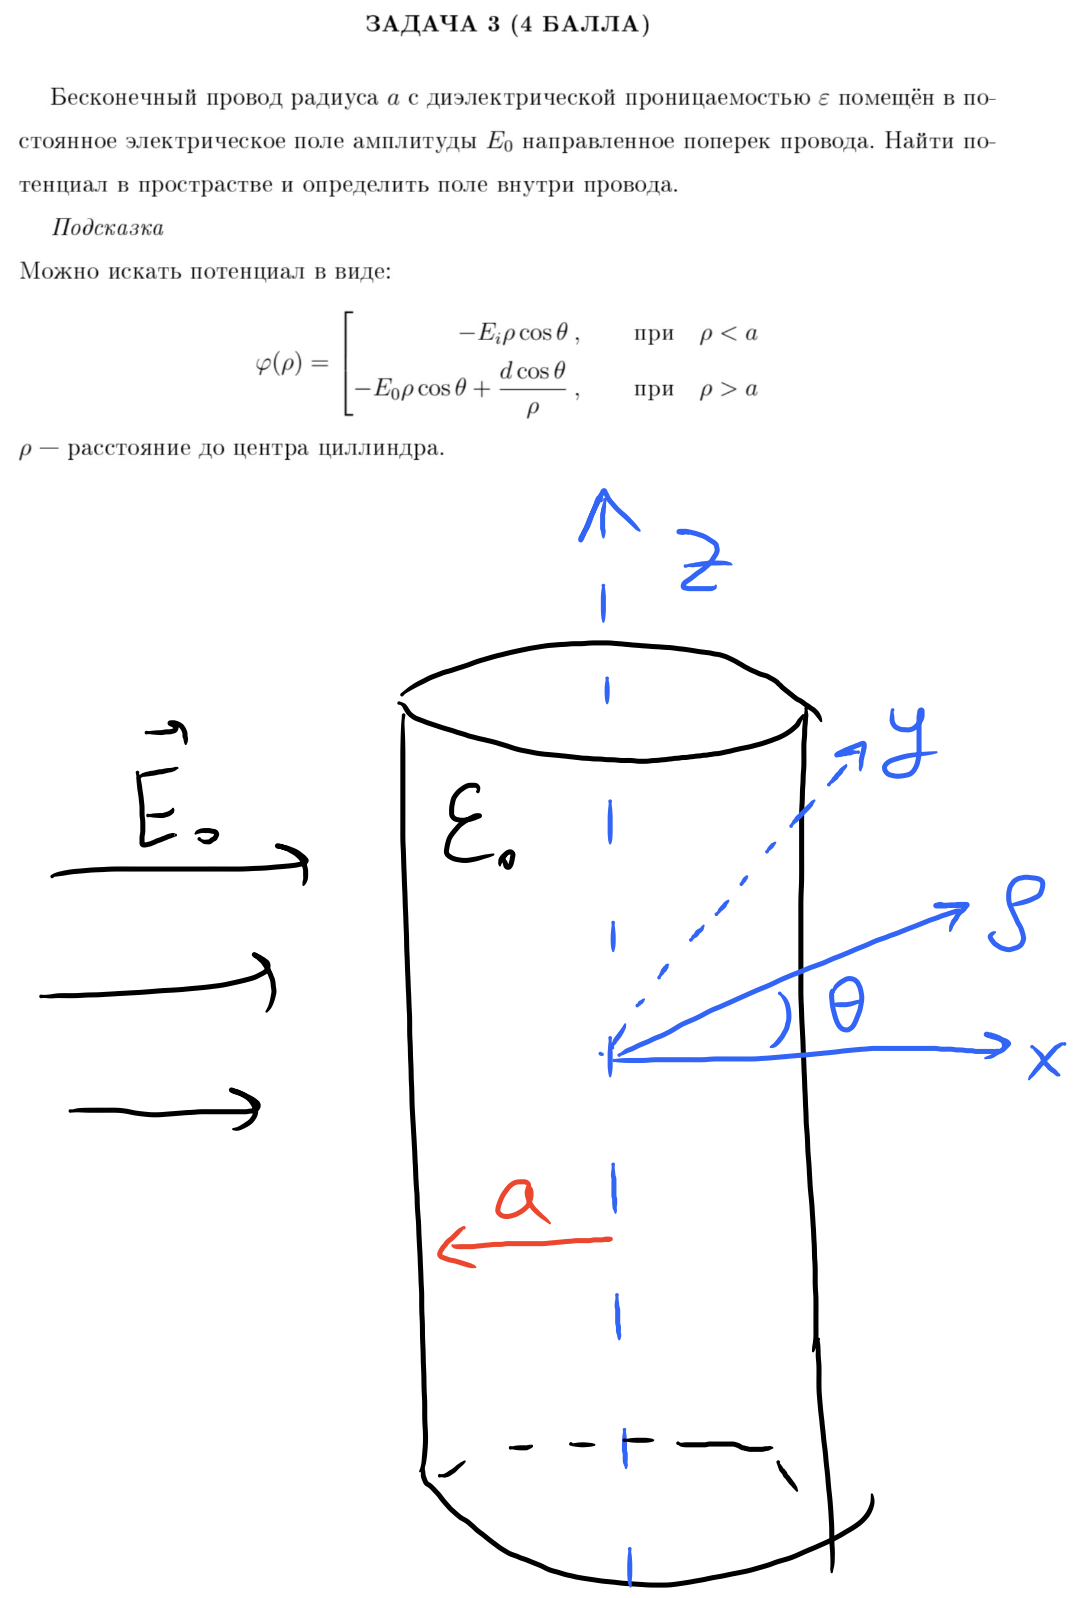
\includegraphics[width=0.5\textwidth]{photo.png}
%\begin{center}
%\underline{Рисунок 1}:
%\end{center}
\par Решение:
\[
    div\left( \overrightarrow{D} \right) = 0 \Rightarrow \overrightarrow{D_{n_1}} = \overrightarrow{D_{n_2}}
\]
\[
    \overrightarrow{D}(\vec{r})=\varepsilon(\vec{r}) \overrightarrow{E}(\vec{r})
\]
\[
    \varepsilon =
    \begin{cases}
        1 ; \rho > a
        \\
        \varepsilon ; \rho \leq a
    \end{cases}
\]
\par На границе:
\[
    E_n\mid_{\rho = a+0} = \varepsilon  E_n\mid_{\rho = a-0}
\]
\[
    \overrightarrow{E} = - \overrightarrow{\nabla} \varphi \Rightarrow E_n = -\frac{\partial \varphi}{\partial \rho}
\]
\par
\[
    \Rightarrow \frac{\partial \varphi}{\partial \rho}\mid_{\rho = a+0} = \varepsilon \frac{\partial \varphi}{\partial \rho}\mid_{\rho = a-0}
\]
\par Так же учтём непрерывность $\varphi$:
\[
    \varphi \mid_{\rho = a+0} =  \varphi \mid_{\rho = a-0}
\]
\par Воспользуемся подсказкой и граничными условиями для нахождения коэффициентов
\[
    \begin{cases}
        -E_0 a \cdot cos(\theta) + \frac{d \cdot cos(\theta)}{a} = -E_i a \cdot cos(\theta)
        \\
        -E_0 \cdot cos(\theta) - \frac{d \cdot cos(\theta)}{a^2} = -E_i \varepsilon \cdot cos(\theta)
    \end{cases}
\]
\par
\[
    \begin{cases}
        -E_0  + \frac{d}{a^2} = -E_i
        \\
        E_0 + \frac{d}{a^2} = E_i \varepsilon
    \end{cases}
\]
\[
    \Rightarrow
    \begin{cases}
        d = \frac{\varepsilon - 1}{\varepsilon + 1}E_0
        \\
        E_i = \frac{2E_0}{\varepsilon + 1}
    \end{cases}
\]
\[
    \Rightarrow  \varphi =
    \begin{cases}
        - \frac{2E_0}{\varepsilon + 1} \rho cos(\theta) ; \rho \leqslant a
        \\
        -E_0 \rho cos(\theta) + \frac{E_0}{\rho}\frac{\varepsilon - 1}{\varepsilon + 1} cos(\theta) ; \rho > a
    \end{cases}
\]
\par В цилиндрических координатах:
\[
    \overrightarrow{\nabla} = \frac{\partial}{\partial \rho} \vec{e_\rho} + \frac{1}{\rho} \frac{\partial}{\partial \varphi} \vec{e_\varphi} + \frac{\partial}{\partial z} \vec{e_z}
\]
\par В силу симметрии задачи по $z \Rightarrow \frac{\partial}{\partial z} = 0$
\[
    \overrightarrow{E}_{\text{внутр}} = - \overrightarrow{\nabla} \varphi ; \text{ при } \rho \leqslant a
\]
\[
    \overrightarrow{E}_{\text{внутр}} = \frac{2E_0}{\varepsilon + 1} cos(\theta) \vec{e_\rho} - \frac{2E_0}{\varepsilon + 1} sin(\theta) \vec{e_\theta}
\]
\par Ответ:
\[
    \varphi =
    \begin{cases}
        - \frac{2E_0}{\varepsilon + 1} \rho cos(\theta) ; \rho \leqslant a
        \\
        -E_0 \rho cos(\theta) + \frac{E_0}{\rho}\frac{\varepsilon - 1}{\varepsilon + 1} cos(\theta) ; \rho > a
    \end{cases}
\]
\[
    \overrightarrow{E}_{\text{внутр}} = \frac{2E_0}{\varepsilon + 1} cos(\theta) \vec{e_\rho} - \frac{2E_0}{\varepsilon + 1} sin(\theta) \vec{e_\theta}
\]
\end{large}
\end{document}
